\section{Модель монополии профсоюза}
\label{sec:monopoly}

Данная модель является моделью отношений профсоюз-фирма по Леонтьеву~\cite{LeontiefW}, в которой профсоюз задаёт уровень заработной платы, после чего фирма выбирает желаемое количество наёмных работников (уровень найма). Предположим что фирма оперирует в условиях конкурентного рынка с рыночной ценой $P$.\\

Порядок игры следующий:\\
\textbf{Первый этап.} Профсоюз устанавливает уровень заработной платы $W$.
\textbf{Второй этап.} Фирма выбирает уровень найма $E$.\\

Выигрыши составляют:\\
Функция полезности профсоюза имеет вид 
$$ U = U(W,E), \quad \frac{\partial U}{\partial W} > 0; \quad \frac{\partial U}{\partial E}~>~0.$$ 
Например $U = \lambda WE.$, где $\lambda \in (0; 1)$\\
Полезность для фирмы измеряется как прибыль 
$$\Pi~=~PY(\bar K,E)~-~WE,$$ 
где цена $P$ дана, а капитал $\bar K$ фиксирован. Отсюда мы можем переписать 
$$\Pi(W,E)~=~R(E)~-~WE,$$ 
где $R$ -- доход.\\

Решение методом обратной индукции:\\
\textbf{Второй этап.} Фирма максимизирует свою прибыль по $L$ при заданном уровне заработной платы. Условие первого порядка примет вид
$$ W = R'(E) = MPE. $$
Разрешая относительно $L$ получим кривую спроса: $E~=~g(W)$.\\
\textbf{Первый этап.} Решается
$$ \max_W U(W,E) = U(W,g(W)). $$
Решение приведено на графике~\ref{fig:monopoly_union}. Графически можно показать, что исход игры неэффективен. Точка $X$ является точкой равновесия обратной индукции модели монополии профсоюза. Точки в закрашенной области Парето-предпочтительнее $X$. $AB$ яаляется кривой контракта, состоящей из точек, в которых изопрофиты и кривые безразличия профсоюза имеют общий тангенс~\cite{ShandongUniver}.


\begin{figure}[h]
		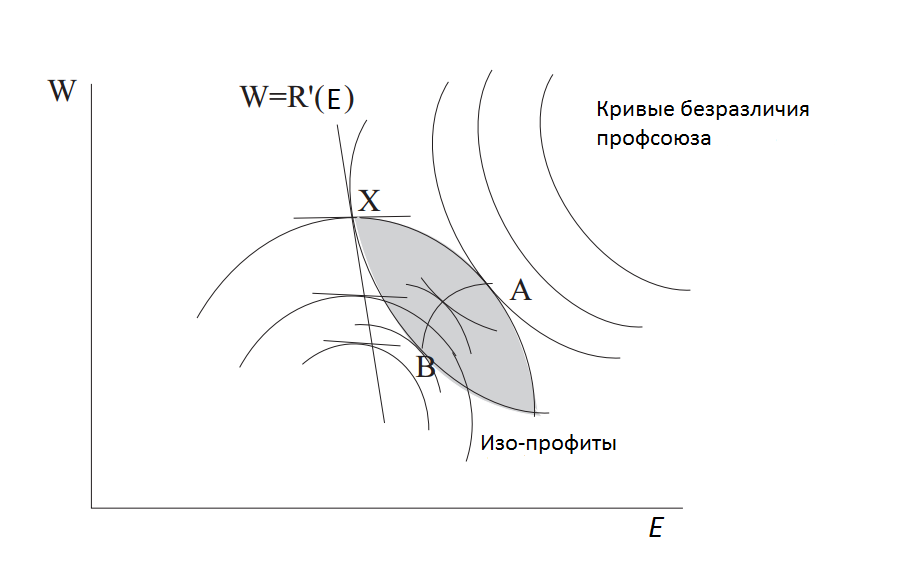
\includegraphics[width=1.0\linewidth]{monopoly_union.png}
		\caption{}
		\label{fig:monopoly_union}
\end{figure}

